% ══════════════════════════════════════════════════════════════════════════════
% 三年研究計畫書（中文，申請教育部獎學金用）— 內容延伸自
% document/industry_academia_collaboration/midterm（僅涵蓋前半年），
% 補充為包含演算法分析與 FPGA 實作之三年研究規劃。
% 編譯方式：LuaLaTeX，見 .latexmkrc；整份申請文件見 ../moe_scholarship.tex
% ══════════════════════════════════════════════════════════════════════════════
\documentclass[11pt,fontset=none]{ctexart}

% ── Packages ──────────────────────────────────────────────────────────────────
\usepackage[margin=0.8in, top=0.7in, bottom=0.8in]{geometry}
\usepackage{amsmath, amssymb}
\usepackage{graphicx}
\usepackage{booktabs}
\usepackage[table]{xcolor}
\usepackage{tabularx}
\usepackage{enumitem}
\usepackage[hidelinks]{hyperref}
\usepackage{caption}
\usepackage{multicol}
\usepackage{float}
\usepackage{tikz}
\usetikzlibrary{positioning, fit, backgrounds, arrows.meta}

% ── Shared fonts and Traditional-Chinese labels ───────────────────────────────
% ══════════════════════════════════════════════════════════════════════════════
% 教育部獎學金申請文件之共用設定（字型與中文標籤）。
% 各份文件以 \documentclass[...,fontset=none]{ctexart} 開頭，再 \input 本檔：
%   % ══════════════════════════════════════════════════════════════════════════════
% 教育部獎學金申請文件之共用設定（字型與中文標籤）。
% 各份文件以 \documentclass[...,fontset=none]{ctexart} 開頭，再 \input 本檔：
%   % ══════════════════════════════════════════════════════════════════════════════
% 教育部獎學金申請文件之共用設定（字型與中文標籤）。
% 各份文件以 \documentclass[...,fontset=none]{ctexart} 開頭，再 \input 本檔：
%   \input{../common/preamble.tex}
% 版面（geometry、行距、頁碼）由各份文件自行設定。
% ══════════════════════════════════════════════════════════════════════════════

% ── CJK font: DFKai-SB (標楷體) on Windows, falling back to AR PL KaitiM Big5
% when DFKai-SB isn't installed (same setup as the midterm report).
\IfFontExistsTF{DFKai-SB}{%
  \setCJKmainfont{DFKai-SB}
  \setCJKsansfont{DFKai-SB}
  \setCJKmonofont{DFKai-SB}
}{%
  \setCJKmainfont{AR PL KaitiM Big5}
  \setCJKsansfont{AR PL KaitiM Big5}
  \setCJKmonofont{AR PL KaitiM Big5}
}

% ── Traditional-Chinese wording overrides ──────────────────────────────────────
\renewcommand{\figurename}{圖}
\renewcommand{\tablename}{表}
\renewcommand{\refname}{參考文獻}

% 版面（geometry、行距、頁碼）由各份文件自行設定。
% ══════════════════════════════════════════════════════════════════════════════

% ── CJK font: DFKai-SB (標楷體) on Windows, falling back to AR PL KaitiM Big5
% when DFKai-SB isn't installed (same setup as the midterm report).
\IfFontExistsTF{DFKai-SB}{%
  \setCJKmainfont{DFKai-SB}
  \setCJKsansfont{DFKai-SB}
  \setCJKmonofont{DFKai-SB}
}{%
  \setCJKmainfont{AR PL KaitiM Big5}
  \setCJKsansfont{AR PL KaitiM Big5}
  \setCJKmonofont{AR PL KaitiM Big5}
}

% ── Traditional-Chinese wording overrides ──────────────────────────────────────
\renewcommand{\figurename}{圖}
\renewcommand{\tablename}{表}
\renewcommand{\refname}{參考文獻}

% 版面（geometry、行距、頁碼）由各份文件自行設定。
% ══════════════════════════════════════════════════════════════════════════════

% ── CJK font: DFKai-SB (標楷體) on Windows, falling back to AR PL KaitiM Big5
% when DFKai-SB isn't installed (same setup as the midterm report).
\IfFontExistsTF{DFKai-SB}{%
  \setCJKmainfont{DFKai-SB}
  \setCJKsansfont{DFKai-SB}
  \setCJKmonofont{DFKai-SB}
}{%
  \setCJKmainfont{AR PL KaitiM Big5}
  \setCJKsansfont{AR PL KaitiM Big5}
  \setCJKmonofont{AR PL KaitiM Big5}
}

% ── Traditional-Chinese wording overrides ──────────────────────────────────────
\renewcommand{\figurename}{圖}
\renewcommand{\tablename}{表}
\renewcommand{\refname}{參考文獻}


% ── Compact spacing so the proposal fits in three pages ───────────────────────
\setlist{itemsep=1pt, topsep=2pt, parsep=0pt}
\ctexset{
  section    = {format=\large\bfseries, beforeskip=8pt, afterskip=3pt},
  subsection = {format=\normalsize\bfseries, beforeskip=5pt, afterskip=2pt},
}
\captionsetup{font=small, skip=3pt}
\setlength{\parskip}{3pt}
\linespread{1.15}\selectfont  % ctex default (1.3) is too loose for a 3-page limit

% Gantt-chart cells: main effort / ramp-up
\newcommand{\G}{\cellcolor{gray!55}}
\newcommand{\Ga}{\cellcolor{gray!25}}

% plain: no running header, page number centered at the bottom
\pagestyle{plain}

\begin{document}

% ── 標頭 ────────────────────────────────────────────────────────────────────────
\begin{center}
  {\Large\bfseries 研究計畫書\par}
  \vspace{2pt}
  {\large 研究主題：合成孔徑雷達（SAR）即時成像演算法——從演算法分析到 FPGA 實作\par}
\end{center}

% ══════════════════════════════════════════════════════════════════════════════
\section{研究背景與動機}

傳統星載合成孔徑雷達（SAR）任務將原始回波下傳至地面站，再於地面完成聚焦成像、影像強化與船舶偵測。由於原始資料量大、下傳頻寬有限，目標資訊送達海事監控端時存在明顯延遲。星載（onboard）處理僅需下傳偵測到的目標資訊，可消除此瓶頸，但受限於衛星酬載之運算能力、記憶體與功耗。此外，SAR 屬同調成像系統，影像中不可避免存在乘性 speckle noise，會造成誤報（false positive）並掩蓋弱散射目標（false negative）。

本研究利用壓縮感測（Compressed Sensing, CS）理論 \cite{donoho_cs, candes_cs}，以同一套輕量化框架同時回應上述兩項問題。海面場景天然具稀疏性：背景均勻、反射率低，船舶則為少數強散射點。場景反射率 $\mathbf{H}$ 由回波 $\mathbf{Y}$ 透過下式重建：
\begin{equation}
  \hat{\mathbf{H}} = \arg\min_{\mathbf{H}} \tfrac{1}{2}\left\|\mathbf{Y} - \mathcal{A}(\mathbf{H})\right\|_F^2 + \lambda R(\mathbf{H}),
  \label{eq:cs}
\end{equation}
其中 $\mathcal{A}(\cdot)$ 為成像前向算子，$R(\cdot)$ 為稀疏誘導正則項。稀疏先驗可將振幅低、以 speckle 為主的背景像素壓制為零，同時保留強目標響應；相較於在特徵層級抑制雜訊之 Transformer 偵測架構 \cite{sares_deim, cvmt}，此方法可採用低複雜度求解器，適合硬體實現。不同於既有稀疏 SAR 成像研究僅以影像品質指標評估 \cite{sparse_sar_imaging, zhang_reweighted, liu_compound_reg}，本研究以\textbf{船舶偵測效能}衡量稀疏成像之實際效益，包括船舶偵測成功率（實際船舶中被正確偵測出的比例）與誤判率（偵測結果中將雜訊誤判為船舶的比例）。

\textbf{總體目標：}發展、分析並以 FPGA 實現一套基於壓縮感測之即時 SAR 成像與船舶偵測處理鏈，使其滿足星載處理器之吞吐量、記憶體與功耗限制，並量化其相對於地面處理之偵測表現。

% ══════════════════════════════════════════════════════════════════════════════
\section{已完成之初步成果}

\begin{itemize}
  \item 評估框架：建立端對端處理鏈——SAR 船舶影像（HRSID \cite{hrsid}）$\to$ 點散射體回波模型 $\to$ CSA（Chirp Scaling Algorithm）成像 \cite{cumming_wong} $\to$ 稀疏精修 $\to$ YOLO 船舶偵測 $\to$ 偵測效能評估。
  \item 單步稀疏精修：在 CSA 成像後，將振幅低於門檻值的像素（多為背景雜訊）壓制為零，僅保留強散射之船舶目標 \cite{sparse_sar_imaging}；於 100 張離岸影像上，整體偵測準確度由 95.4\%（僅 CSA）提升至 98.5\%，範例如圖 \ref{fig:refinement}。
  \item GPU 加速模擬：回波模擬需逐一計算每個散射點於每個取樣時間之貢獻，大量影像之評估極為耗時；因此將回波產生與 CSA 成像移至 GPU 平行運算，回波產生速度較 24 核心 CPU 快約 580 倍，使全資料集評估得以實現。
  \end{itemize}

\begin{figure}[H]
  \centering
  \begin{minipage}{0.24\textwidth}
    \centering
    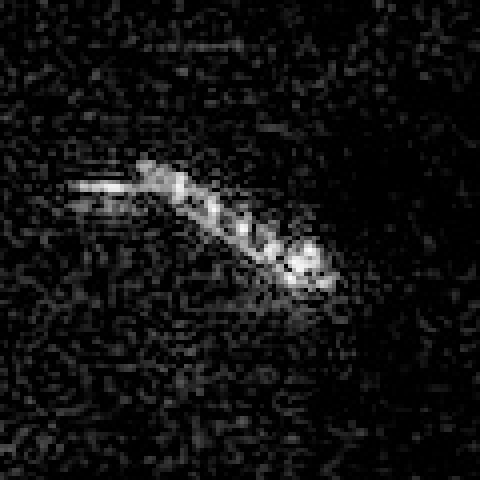
\includegraphics[width=\linewidth]{figures/detection_csa.png}
    \caption*{傳統成像（CSA）}
  \end{minipage}
  \hspace{0.04\textwidth}
  \begin{minipage}{0.24\textwidth}
    \centering
    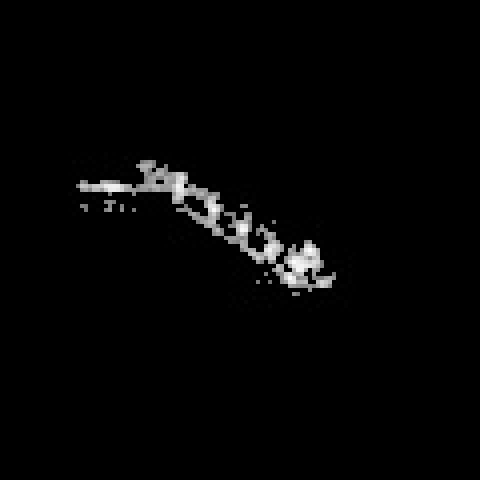
\includegraphics[width=\linewidth]{figures/detection_csa_threshold.png}
    \caption*{本研究方法（CSA + 稀疏精修）}
  \end{minipage}
  \caption{稀疏精修範例。傳統成像之海面背景雜訊明顯；稀疏精修利用場景稀疏性將背景雜訊壓制為零，同時保留船體結構。}
  \label{fig:refinement}
\end{figure}

% ══════════════════════════════════════════════════════════════════════════════
\section{三年研究規劃}

本研究分為三個階段，由演算法設計、硬體導向之演算法分析，逐步推進至 FPGA 原型實作，研究架構如圖 \ref{fig:arch}：上方為研究標的——星載即時成像與偵測處理鏈，下方三層為各年度工作項目，前一年度之成果作為下一年度之輸入；各項工作之時程如圖 \ref{fig:gantt}。

\begin{figure}[tbp]
  \centering
  \begin{tikzpicture}[
      font=\footnotesize,
      chain/.style={draw, rounded corners=2pt, align=center, minimum width=2.5cm,
                    minimum height=0.8cm, fill=blue!8},
      task/.style={draw, rounded corners=2pt, align=center, minimum width=3.9cm,
                   minimum height=0.65cm, fill=white, inner sep=2pt},
      yr/.style={align=center, minimum width=1.7cm, font=\footnotesize\bfseries},
      arr/.style={-{Stealth[length=2mm]}, thick},
      band/.style={draw, rounded corners=4pt, inner sep=4pt},
    ]
    % ── 研究標的：星載處理鏈 ──
    \node[chain] (c1) at (0.05,0)  {回波模擬};
    \node[chain] (c2) at (3.05,0)  {SAR 成像};
    \node[chain] (c3) at (6.05,0)  {稀疏重建};
    \node[chain] (c4) at (9.05,0)  {船舶偵測};
    \node[chain] (c5) at (12.05,0) {偵測表現評估};
    \foreach \a/\b in {c1/c2, c2/c3, c3/c4, c4/c5} \draw[arr] (\a) -- (\b);
    \draw[arr, dashed] (c5.north) -- ++(0,0.3) -| node[pos=0.25, above]{回饋演算法選擇} (c3.north);
    % ── 年度工作 ──
    \foreach \y/\lab/\col/\ta/\tb/\tc [count=\i] in {
        -1.35/第一年\\演算法發展/green!8/Speckle 建模與模擬/稀疏正則化方法比較/去斑方法比較,
        -2.45/第二年\\演算法分析/orange!10/迭代式壓縮感測成像/運算複雜度分析/硬體導向演算法簡化,
        -3.55/第三年\\FPGA 實作/red!8/成像電路實作/偵測模型硬體部署/系統驗證與效能量測} {
      \coordinate (L\i) at (-1.15,\y);
      \node[yr] (l\i) at (-0.3,\y) {\lab};
      \node[task] (t1\i) at (2.75,\y)  {\ta};
      \node[task] (t2\i) at (7.05,\y)  {\tb};
      \node[task] (t3\i) at (11.35,\y) {\tc};
      \begin{scope}[on background layer]
        \node[band, fill=\col, fit=(L\i)(t1\i)(t3\i)] (b\i) {};
      \end{scope}
    }
  \end{tikzpicture}
  \caption{研究架構圖：上方為星載即時成像與偵測處理鏈，下方為三年度之工作項目。}
  \label{fig:arch}
\end{figure}

\subsection{第一年：演算法發展}
\begin{enumerate}[label=(\arabic*), leftmargin=2.2em]
  \item Speckle 建模與模擬：以真實星載 SAR 影像統計 speckle 雜訊之分布特性，將其加入回波模擬中，使模擬資料更貼近實際衛星影像。
  \item 稀疏正則化方法比較：比較多種稀疏正則化方法 \cite{zhang_reweighted, liu_compound_reg}，並依海面背景之統計特性自動決定門檻值，取代人工設定之固定門檻。
  \item 去斑方法比較：將稀疏重建與傳統去斑濾波器（如 Lee 濾波器）比較，同時以影像品質與船舶偵測表現評估，並分別探討近岸與離岸場景。
\end{enumerate}

\subsection{第二年：演算法分析}
\begin{enumerate}[label=(\arabic*), leftmargin=2.2em]
  \item 迭代式壓縮感測成像：由第一年之「成像後再稀疏化」延伸為直接由回波進行迭代式稀疏重建 \cite{fista, fang_approx_obs}，並探討在減少取樣資料量的情況下，是否仍能維持偵測表現，以降低星上資料量與運算需求。
  \item 運算複雜度分析：分析成像與重建演算法所需之運算量、記憶體用量與迭代次數，找出偵測準確率與處理速度之間的最佳平衡。
  \item 硬體導向演算法簡化：以有限位元數模擬硬體運算，評估精度降低對成像品質與偵測結果之影響；並將偵測模型輕量化，使其適合在資源有限之硬體上執行。
\end{enumerate}

\subsection{第三年：FPGA 實作}
\begin{enumerate}[label=(\arabic*), leftmargin=2.2em]
  \item 成像電路實作：將 SAR 成像與稀疏重建之主要運算（如快速傅立葉轉換、相位補償、門檻化）設計為 FPGA 硬體電路，並規劃大量影像資料於記憶體中之存取方式。
  \item 偵測模型硬體部署：將輕量化之船舶偵測模型部署於同一 FPGA 平台，與成像電路串接為完整之星上處理流程，最終僅輸出偵測到的船舶資訊。
  \item 系統驗證與效能量測：以模擬資料及真實衛星資料驗證硬體結果與軟體模型一致，並量測處理速度、延遲、硬體資源用量與功耗，與 CPU/GPU 實作比較；最後整理研究成果並發表論文。
\end{enumerate}

\newpage
% ══════════════════════════════════════════════════════════════════════════════
\section{預期貢獻}

（1）提出以船舶偵測準確率而非僅以影像品質指標衡量稀疏 SAR 成像之任務導向評估方法；（2）分析壓縮感測 SAR 成像在準確率、運算複雜度與字長之間的折衷關係；（3）完成 FPGA 原型，證明星載壓縮感測成像結合船舶偵測可於衛星酬載限制內實現，使下傳資料量降至僅需目標報告。

% ══════════════════════════════════════════════════════════════════════════════
\section{時程與查核點}

\begin{figure}[H]
  \centering
  \footnotesize
  \setlength{\tabcolsep}{2.2pt}
  \renewcommand{\arraystretch}{0.95}
  \begin{tabular}{l@{\hspace{8pt}}*{12}{>{\centering\arraybackslash}p{1.1em}}}
    \toprule
     & \multicolumn{4}{c}{第一年} & \multicolumn{4}{c}{第二年} & \multicolumn{4}{c}{第三年} \\
    \cmidrule(lr){2-5}\cmidrule(lr){6-9}\cmidrule(lr){10-13}
    工作項目（季） & 1 & 2 & 3 & 4 & 1 & 2 & 3 & 4 & 1 & 2 & 3 & 4 \\
    \midrule
    Speckle 建模與模擬     & \G & \G & \Ga & & & & & & & & & \\
    稀疏正則化方法比較     & & \G & \G & \G & & & & & & & & \\
    去斑方法比較           & & & \G & \G & & & & & & & & \\
    迭代式壓縮感測成像     & & & & \Ga & \G & \G & & & & & & \\
    運算複雜度分析         & & & & & \G & \G & \G & & & & & \\
    硬體導向演算法簡化     & & & & & & \G & \G & \G & & & & \\
    成像電路實作           & & & & & & & & \Ga & \G & \G & \G & \\
    偵測模型硬體部署       & & & & & & & & & \G & \G & \G & \\
    系統驗證與效能量測     & & & & & & & & & & \G & \G & \G \\
    \bottomrule
  \end{tabular}
  \caption{三年時程甘特圖（深色：主要工作期間，淺色：前置/交疊期間）。}
  \label{fig:gantt}
\end{figure}

\begin{table}[H]
  \centering
  \footnotesize
  \caption{查核點與交付成果。}
  \label{tab:milestones}
  \begin{tabularx}{\textwidth}{c l X}
    \toprule
    年度 & 查核點 & 交付成果 \\
    \midrule
    1 & 含 speckle 之評估框架 & 經實際資料驗證之 speckle 模型；以星載參數完成近岸與離岸影像之模擬 \\
      & 演算法比較 & 完成稀疏正則化方法與傳統去斑濾波器於偵測表現上之比較 \\
    \midrule
    2 & 迭代式壓縮感測成像 & 完成由降取樣回波之壓縮感測重建，並分析取樣率對偵測表現之影響 \\
      & 硬體導向演算法 & 完成定點數模型與輕量化偵測模型，並建立硬體原型 \\
    \midrule
    3 & FPGA 原型 & 成像與船舶偵測於 FPGA 平台上運行 \\
      & 系統驗證 & 完成吞吐量、延遲、資源與功耗量測並與 CPU/GPU 比較；期刊/研討會論文發表 \\
    \bottomrule
  \end{tabularx}
\end{table}

% ══════════════════════════════════════════════════════════════════════════════
\begin{multicols}{2}
\footnotesize
\begin{thebibliography}{99}
\setlength{\itemsep}{0pt}

\bibitem{donoho_cs}
D. L. Donoho, ``Compressed Sensing,'' \textit{IEEE Trans. Inf. Theory}, vol. 52, no. 4, pp. 1289--1306, 2006.

\bibitem{candes_cs}
E. J. Cand\`es \textit{et al.}, ``Robust Uncertainty Principles: Exact Signal Reconstruction from Highly Incomplete Frequency Information,'' \textit{IEEE Trans. Inf. Theory}, vol. 52, no. 2, pp. 489--509, 2006.

\bibitem{sares_deim}
F. Song \textit{et al.}, ``SARES-DEIM: Sparse Mixture-of-Experts Meets DETR for Robust SAR Ship Detection,'' \textit{IEEE JSTARS}, 2026.

\bibitem{cvmt}
K. Ni \textit{et al.}, ``Complex-Value Transformer for SAR Ship Detection,'' \textit{ISPRS J. Photogramm. Remote Sens.}, 2026.

\bibitem{sparse_sar_imaging}
H. Bi \textit{et al.}, ``From Theory to Application: Real-Time Sparse SAR Imaging,'' \textit{IEEE Trans. Geosci. Remote Sens.}, vol. 58, no. 4, pp. 2928--2936, 2020.

\bibitem{zhang_reweighted}
Y. Zhang \textit{et al.}, ``Undistorted and Consistent Enhancement of Automotive SAR Image via Multi-Segment-Reweighted Regularization,'' \textit{Remote Sens.}, vol. 17, no. 9, 1483, 2025.

\bibitem{liu_compound_reg}
M. Liu \textit{et al.}, ``A Sparse SAR Imaging Method for Low-Oversampled Staggered Mode via Compound Regularization,'' \textit{Remote Sens.}, vol. 16, no. 8, 1459, 2024.

\bibitem{hrsid}
S. Wei \textit{et al.}, ``HRSID: A High-Resolution SAR Images Dataset for Ship Detection and Instance Segmentation,'' \textit{IEEE Access}, vol. 8, pp. 120234--120254, 2020.

\bibitem{cumming_wong}
I. G. Cumming and F. H. Wong, \textit{Digital Processing of Synthetic Aperture Radar Data: Algorithms and Implementation}, Artech House, 2005.

\bibitem{fista}
A. Beck and M. Teboulle, ``A Fast Iterative Shrinkage-Thresholding Algorithm for Linear Inverse Problems,'' \textit{SIAM J. Imaging Sci.}, vol. 2, no. 1, pp. 183--202, 2009.

\bibitem{fang_approx_obs}
J. Fang \textit{et al.}, ``Fast Compressed Sensing SAR Imaging Based on Approximated Observation,'' \textit{IEEE JSTARS}, vol. 7, no. 1, pp. 352--363, 2014.

\end{thebibliography}
\end{multicols}

\end{document}
